\documentclass[border=0.2cm]{standalone}
\usepackage{tikz}
\begin{document}


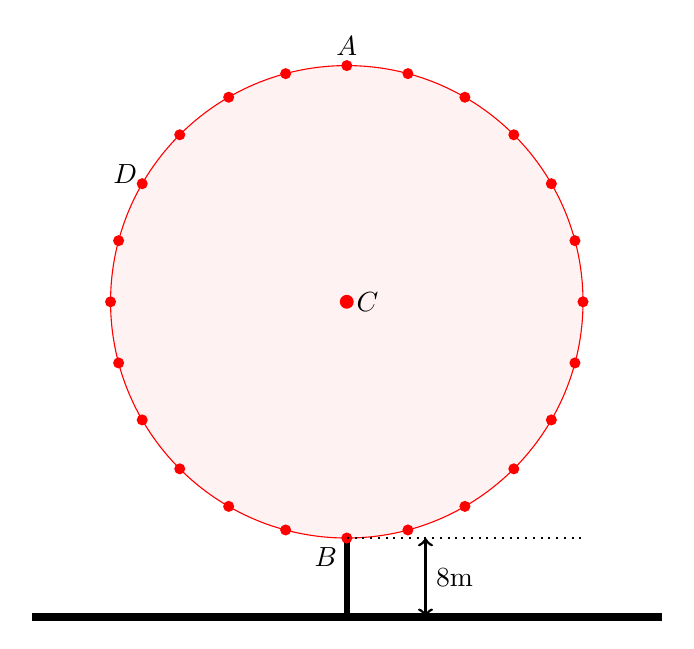
\begin{tikzpicture}
  %\draw[help lines,black!30] (-5.5,-5.5) grid (5.5,5.5);
  %\draw[thick,->] (0,-5) -- (0,5) node[left]  {$y$};
  %\draw[thick,->] (-5,0) -- (5,0) node[below] {$x$};
  %\foreach \x in {-4,-3,-2,-1,1,2,3,4} \node[left,color=red] at (0,\x) {\x} node[below,color=red] at (\x,0) {\x};
  %\node[below right,color=red] at (0,0) {0}; 

\draw[line width=2pt] (0,-4) -- (0,0);
\draw[fill=red!5,draw=red] (0,0) circle (3);

\foreach \x in {15,30,...,360} {\fill[red] (\x:3) circle (2pt);}
\fill[red] (0,0) circle (2.5pt);
\draw[dotted, thick] (0,-3) -- (3,-3);
\draw[line width=1pt, <->] (1,-3) -- (1,-4) node[midway,right] {8m};
\draw[line width=3pt] (-4,-4) -- (4,-4);
\node[above] at (90:3) {$A$};
\node[below left] at (0,-3) {$B$};
\node[right] at (0,0) {$C$};
\node at (150:3.25) {$D$};

\end{tikzpicture}



\end{document}